\documentclass[main]{subfiles}
\begin{document}

%@@@@@@@@@@@@@@@@@@@@@@@@@@@@@@
% summarizes lecture 2
% author: David Bontrager

%David:
\section{Subthreshold behavior}
Depending on how we want a transistor to behave, we will want to keep it in subthreshold. A few of the biggest reasons to do so are low power consumption (nano- or microamps), less dominant Early voltage effects, and the usefulness of logarithmic behavior (can cover many orders of magnitude of current for less than one order of magnitude of voltage). Most circuits in this class involve subthreshold transistors, so these are extremely important concepts to understand. In this chapter I will discuss only nFET transistors. To do the equations for pFET devices, you simply multiply all voltages by $-1$\footnote{We did not previously mention this, but pFET bulks are tied to $V_{dd}$, not ground, so all voltages are relative to that (that is, the relevant $V_{g}$ for a pFET would be calculated as $V_{dd} - V_{g}$). The same goes for drain and source voltages. Generally, what the bulk is tied to is hard-wired into the device, though sometimes we make a device where there is a fourth lead controlling this.}.
%-----------------------------------------------
\subsection{On subs, threshes, and holds}
Yeah it's a bad section title. Don't worry about it. We mentioned $\kappa$ above. It's pretty darn important, so let's look at the mathematical definition:
\begin{equation}
\kappa = \frac{C_{ox}}{C_{ox} + C_{dep}} = \frac{\partial\psi_s}{\partial V_g}
\label{kappaEqn}
\end{equation}
where $C_{ox}$ is the capacitance across the insulating oxide and $C_{dep}$ is the capacitance across the depletion layer, as illustrated in Figure~\ref{crossSectionCaps}. $\psi_s$ is a function of a number of terms, but this is what it boils down to and why it is important\footnote{p.44 in the textbook has details on how the partial derivative comes into play, but the lecture slides do a better job of making this point}. Typical values for $\kappa$ are between 0.4 and 0.9, though it clearly must - mathematically - be less than 1 (look at ~\eqref{kappaEqn}) \\ \\
%-------MOSFET circuit diagram--------
\begin{figure}[ht]
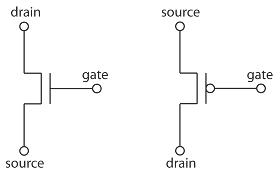
\includegraphics[natwidth=560,natheight=350]{figs/nme_mosfets.pdf}
\caption{Circuit diagrams for an nFET (left) and a pFET (right). Terminals are labeled such that, in a standard circuit diagram, $V_{dd}$ is above the components and $ground$ is below them. However, nothing in the device forces it to be this way. They are physically symmetric and can work with current flowing in either direction. \label{mosfetsFig}}
\end{figure}
%-------------------------------------
Okay, so we're subthreshold. $V_{gs}$ is low but non-zero. Let's say the source and drain, both of which are $n$-type material sitting in the $p$-type substrate, are also both at $0V$ relative to ground. Because of the low gate voltage, the electrons have an energy barrier to overcome\footnote{That's not the best way to put it. The built-in potential from the $pn$ junctions creates the energy barrier. This voltage will be such that the $n$-type material (drain and source in an nFET) is at a higher voltage than the $p$-type material (the substrate in an nFET), so due to the electric field electrons want to flow from $p$-type to $n$. If we then increase $V_g$, the positive charge on the gate pushes the \emph{substrate's} mobile carriers (holes) away from the silicon oxide, leaving a negatively-charged depletion region immediately under the surface. This is the channel where we see inversion - this is how we form the inversion layer. Broadening this channel (increasing $V_g$) makes it take less energy for an electron to move from the drain or source into the channel, and \emph{that} is what's happening with the energy barrier.} if they want to travel between drain or source and the channel. It's difficult - the natural state is quite resistive. Raising the gate voltage (but keeping it under 0.7V, the approximate threshold voltage) means electrons can more easily move through the channel because the energy barrier is lower. But they have no reason to move. It is not more favorable energy-wise to be at the source compared to being at the drain, because drain-source voltage is still zero.\\ \\
We raise the drain voltage, though only a little. Tens of millivolts. The drain side now has a slightly higher energy barrier for its electrons to cross if they want to enter the channel\footnote{This energy barrier stuff takes a little thinking to get used to, but soon you don't worry about this because you only care about the ``what,'' not the ``why.'' They spend a reasonable amount of time on it in class, so pay attention and ask questions and it should make sense}. The mobile carrier concentration at either end of the channel is a function of this barrier height. If we change the barrier height at one end and not the other, carrier concentration will decrease on the side with the higher barrier, setting up a concentration gradient. What do we know happens across gradients? Yes! Diffusion! \emph{This is important to note – the electric field across the channel is still not the main driving force in current flow. Electrons are moving primarily due to the concentration gradient.} Sure, it's only tens or hundreds of nanoamps, but it's current!\\ \\
Current flows with even very small drain-source voltages. For a small range of voltages, it stays in the \emph{triode/ohmic/linear} region. The name comes from the fact that current has an approximately \emph{linear} dependence on drain-source voltage \emph{when the transistor is above threshold}\footnote{The ``ohmic'' part of the name is simply projecting Ohm's law on the linear regime, describing the fact that the transistor acts as linear (ohmic) resistor in that range. That is, current increases linearly with voltage, just like $V=IR$ says.}. In fact it is also approximately linear while subthreshold for $V_{ds}$ below $U_T$\footnote{about 25 mV, remember?}, but then the exponential starts kicking in. To be clear, it only looks linear instead of exponential here \emph{because the exponential itself behaves linearly} over a small range. It's a math thing. Once you get above $4U_T$ (about 100mV), you enter the saturation region, where current is nearly constant across any higher drain-source voltage for a given gate voltage. This means that operating in subthreshold saturation region is an easy way to get a constant current source if you can set your gate and source voltages and you are unsure about what your drain voltage will be (as long as it stays above $4U_T$, the drain voltage can move around without affecting the output current).\\ \\
We could go through all the derivations for getting the drain-source current equations, but we'll leave that to the textbook. You start with current as a function of electron diffusion current density, channel width, and channel depth\footnote{Equation 3.2.5, p. 55}. The diffusion current density is a function of electron mobility and the concentration gradient across the channel. So we calculus-up our equations, and end up with a few constants prefixing a couple exponential terms raised to the power of various voltages and our old friend $\kappa$. It looks like this:
\begin{equation}
I = I_0 e^{(\kappa V_g - V_s)/U_T} - I_0 e^{(\kappa V_g - V_{d})/U_T}
\label{subTriodeEqn}
\end{equation}
Now we see why it flattens out onces $V_{ds}$ goes above $4U_T$ - the second term becomes negligible and thus the output does not change for higher $V_{ds}$. The form for ~\eqref{subTriodeEqn} comes from the fact that the total current ($I$) is the difference between the forward current (the first term) and the reverse current (the second term). A different form is
\begin{equation}
I = I_0 e^{(\kappa V_g - V_s)/U_T}(1 - e^{-V_{ds}/U_T})
\end{equation}
We've already said it, so we might as well come out with the equation for a transistor in subthreshold \emph{saturation}. Remember, this applies when $V_{ds} > 4U_T$ (in saturation) and $V_{gs} < 0.7V$ (subthreshold).
\begin{equation}
I = I_0 e^{(\kappa V_g - V_s)/U_T} \label{subSatEqn}
\end{equation}
or, since we often tie $V_s$ to ground:
\begin{equation}
I = I_0 e^{\kappa V_g/U_T}
\end{equation}
Spend some time looking at the plots in the textbook and the lecture slides - that will help you get a sense for what is different and what changes when you play with the inputs on a transistor\footnote{Figs 3.6-3.8, pp. 58-60, and Fig 3.10, p. 63}. \textsl{An important point: as long as they're in \emph{subthreshold}, transistors always go between saturation and triode regimes at $V_{ds} = 4U_T$, regardless of $V_{gs}$. However, an \emph{above threshold} transistor's transition $V_{ds}$ to go between triode and saturation regimes \emph{does} change for different values of $V_{gs}$.}\footnote{In all of these cases, we keep $V_{gs}$ constant while sweeping $V_{ds}$, and then repeat for a different value of $V_{gs}$}\\ \\
The constant ``$I_0$'' is just a bunch of other constants smushed together for convenience and because we're rather embarrassed by them. No self-respecting physicist wants half a dozen consecutive constants sullying their equations, so you clean it up with a compound constant\footnote{If you want the details: Equation 3.2.7, p. 56}. The only part that we need to remember for later is that it includes the transistor dimension ratio $\frac{W}{L}$ for channel width ($W$) and length ($L$).\\ \\
At some point we will want to calculate $\kappa$. One easy way is, for an nFET, to tie the drain to $V_{dd}$, tie the source to ground through an ammeter (like the Keithley 236 SMU), and sweep the gate voltage from $0V$ to $1.2V$ or a similar range. Plotting the output current on a \texttt{semilogy} plot (log of measured current on y-axis, gate voltage on x-axis) gives a curve where, in the linear regime, the slope is $\kappa/U_T$.
%------Lab 2, Experiment 1 - Ids vs Vg----------
\begin{figure}[ht]
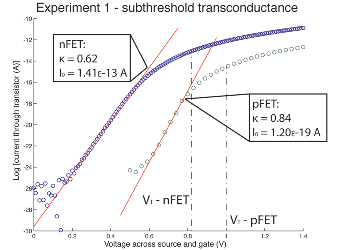
\includegraphics[natwidth=675,natheight=500]{figs/nme_lab2exp1.pdf}
\caption{Reasonable-looking results from lab 2 - measuring $\kappa$ and threshold voltage as described in class (slope of red lines is $\kappa/U_T$) \label{lab2exp1}}
\end{figure}
%-----------------------------------------------
\subsection{On conductance, Early voltage, and mismatch}
Not all transistors behave exactly the same. In fact, it's not easy to find two that do. We call this \emph{device mismatch}. It's primarily a function of the randomness involved in the doping procedure, which is a diffusion process. Because of this, we cannot ensure that any two transistors have the same response characteristics without testing them and finding two that are close enough. We simply cannot control the process that well. There is also uncertainty with dimension tolerances\footnote{In any manufacturing process, a dimension will be produced to a tolerance of $\pm\varepsilon$, so this inherent variation in physical dimensions is going to change the behavior of the transistor ($I_0$ is a function of width and length, remember?)}.\\ \\
This becomes a problem if you design a circuit that is very sensitive to device response characteristics and relies on symmetry between certain devices within the circuit. There are ways to mediate or minimize the problem, but  basically it manifests itself as deviation from an ideal behavior (lateral translation of output vs input plots, threshold variation, etc).\\ \\
Another non-ideal behavior of transistors produces what we call the \emph{Early voltage}\footnote{Named after a person, not a temporal relation}. We said earlier that a transistor does not increase its output current for higher \emph{drain-source} voltages after passing the saturation voltage. This is not actually true, especially for short length MOSFETs. In the above threshold saturation regime, increasing drain voltage beyond the saturation point extends the pinchoff region\footnote{See p. 67, ``Saturation Region'' section for a description of the \emph{pinchoff region}. Really, all you need to remember about the Early voltage is 1) what it does to your output, 2) how to calculate it, and 3) that it's more pronounced in short transistors} further into the channel away from the drain, decreasing the effective length of the transistor and thus increasing its output current. To calculate it, you simply measure the current through a transistor while sweeping the drain voltage. Extrapolate a line from where the saturation region has flattened out and see where it hits the x-axis. This will be the negative Early voltage\footnote{See p.76, Fig 3.16}. The slope of this line is also the \emph{drain conductance} of the transistor at this point, represented as
\begin{equation}
g_{ds} = \frac{\partial I_{ds}}{\partial V_{ds}} = \frac{I}{V_e}
\label{gDrainEqn}
\end{equation}
\\
As transistor length increases, so does Early voltage. The ideal transistor would have an Early voltage of $V_e = \infty$ (horizontal slope, no x-intercept). More imperfections are discussed in the textbook section 3.5 (p. 75), but these are the most important two. It's good to be aware of the other effects (and you have to discuss them in one or two of the lab writeups), but they make fewer appearances throughout the course. The important thing is to understand how mismatch can affect your circuit and what kind of change in behavior you would expect to see for mismatch showing up in any given transistor.\\ \\
While \emph{conductance} is on our minds, let's spend another minute on it. We do know what it is in a general sense - it's $R^{-1}$, right? The inverse of the resistance? If $V = IR$, then $R = V/I$ and $g = I/V$. This is all just a very general statement from our old friend Ohm's Law with no transistor-specific properties. These relationships are a little more involved in transistors than in normal, linear resistors, so we take a more dynamic view and call the conductance the partial derivative of the drain current in terms of the voltage of whichever terminal we're interested in. We tend not to move the source around too much, so mostly we talk about the drain conductance, as shown in ~\eqref{gDrainEqn}, and the gate conductance, most often called the \emph{transconductance}. We call it the transconductance because the current we are concerned with does not go through the terminal whose voltage we are changing\footnote{Remember, it's the gate, and no current goes in or out of the gate}.
\begin{equation}
g_{m} = \frac{\partial I}{\partial V_{g}}
\label{gTransEqn}
\end{equation}
To get conductance expressions, you simply differentiate your relevant current equation, like ~\eqref{subSatEqn}, in terms of the relevant voltage.\\ \\
That pretty well covers the basics of subthreshold behavior, though probably not everything. I didn't plan this thing out all that well. There's also some stuff about $\kappa$ not actually being constant, but you'll see that in the labs.
%-----------------------------------------------
\end{document}